% =============================================================================
% 5. OBSERVABILIDAD
% =============================================================================
\section{Observabilidad}
\label{sec:observability}

\subsection{Stack LGTM con OpenTelemetry}

Para monitorear el servicio en producci\'on se implement\'o un stack de observabilidad completo basado en el proyecto open-source \textbf{Grafana LGTM} (Loki, Grafana, Tempo, Mimir) con OpenTelemetry como capa de instrumentaci\'on. La Tabla~\ref{tab:observability-stack} describe cada componente:

\begin{table}[H]
\centering
\caption{Componentes del stack de observabilidad.}
\label{tab:observability-stack}
\small
\begin{tabularx}{\textwidth}{llX}
\toprule
\textbf{Componente} & \textbf{Se\~nal} & \textbf{Prop\'osito} \\
\midrule
Tempo      & Traces   & Tracing distribuido: latencia por endpoint, spans por request \\
Loki       & Logs     & Agregaci\'on de logs estructurados del backend \\
Mimir      & Metrics  & M\'etricas de rendimiento (throughput, latencia p95, errores) \\
Pyroscope  & Profiles & Profiling continuo de CPU/memoria (flame graphs) \\
Grafana    & ---      & Visualizaci\'on unificada de todas las se\~nales \\
OTel Collector & --- & Recepci\'on y enrutamiento de telemetr\'ia via OTLP \\
\bottomrule
\end{tabularx}
\end{table}

\subsection{Instrumentaci\'on del backend}

La instrumentaci\'on se implementó con el SDK de OpenTelemetry para Python, configurable din\'amicamente mediante la variable de entorno \texttt{OTEL\_ENABLED}:

\begin{itemize}
    \item \textbf{Traces}: auto-instrumentaci\'on de FastAPI genera spans por cada request HTTP con m\'etodo, ruta, status code y duraci\'on.
    \item \textbf{Logs}: el handler de OTel se conecta al \texttt{logging} de Python, exportando todos los logs INFO/WARNING/ERROR a Loki via OTLP.
    \item \textbf{Metrics}: m\'etricas HTTP est\'andar (request count, latencia, tama\~no) m\'as m\'etricas custom de negocio.
\end{itemize}

\noindent
M\'etricas custom implementadas:

\begin{itemize}
    \item \texttt{chest\_xpert.predictions\_total}: contador de predicciones realizadas.
    \item \texttt{chest\_xpert.inference\_duration\_seconds}: histograma de duraci\'on de inferencia ONNX.
\end{itemize}

\subsection{Despliegue con Docker Compose}

El stack se levanta con un solo comando mediante \texttt{docker compose up}, desplegando dos contenedores:

\begin{lstlisting}[language=bash, caption={Levantar el stack completo.}]
docker compose up -d
# API:     http://localhost:8000
# Grafana: http://localhost:3000 (admin/admin)
\end{lstlisting}

\begin{figure}[H]
    \centering
    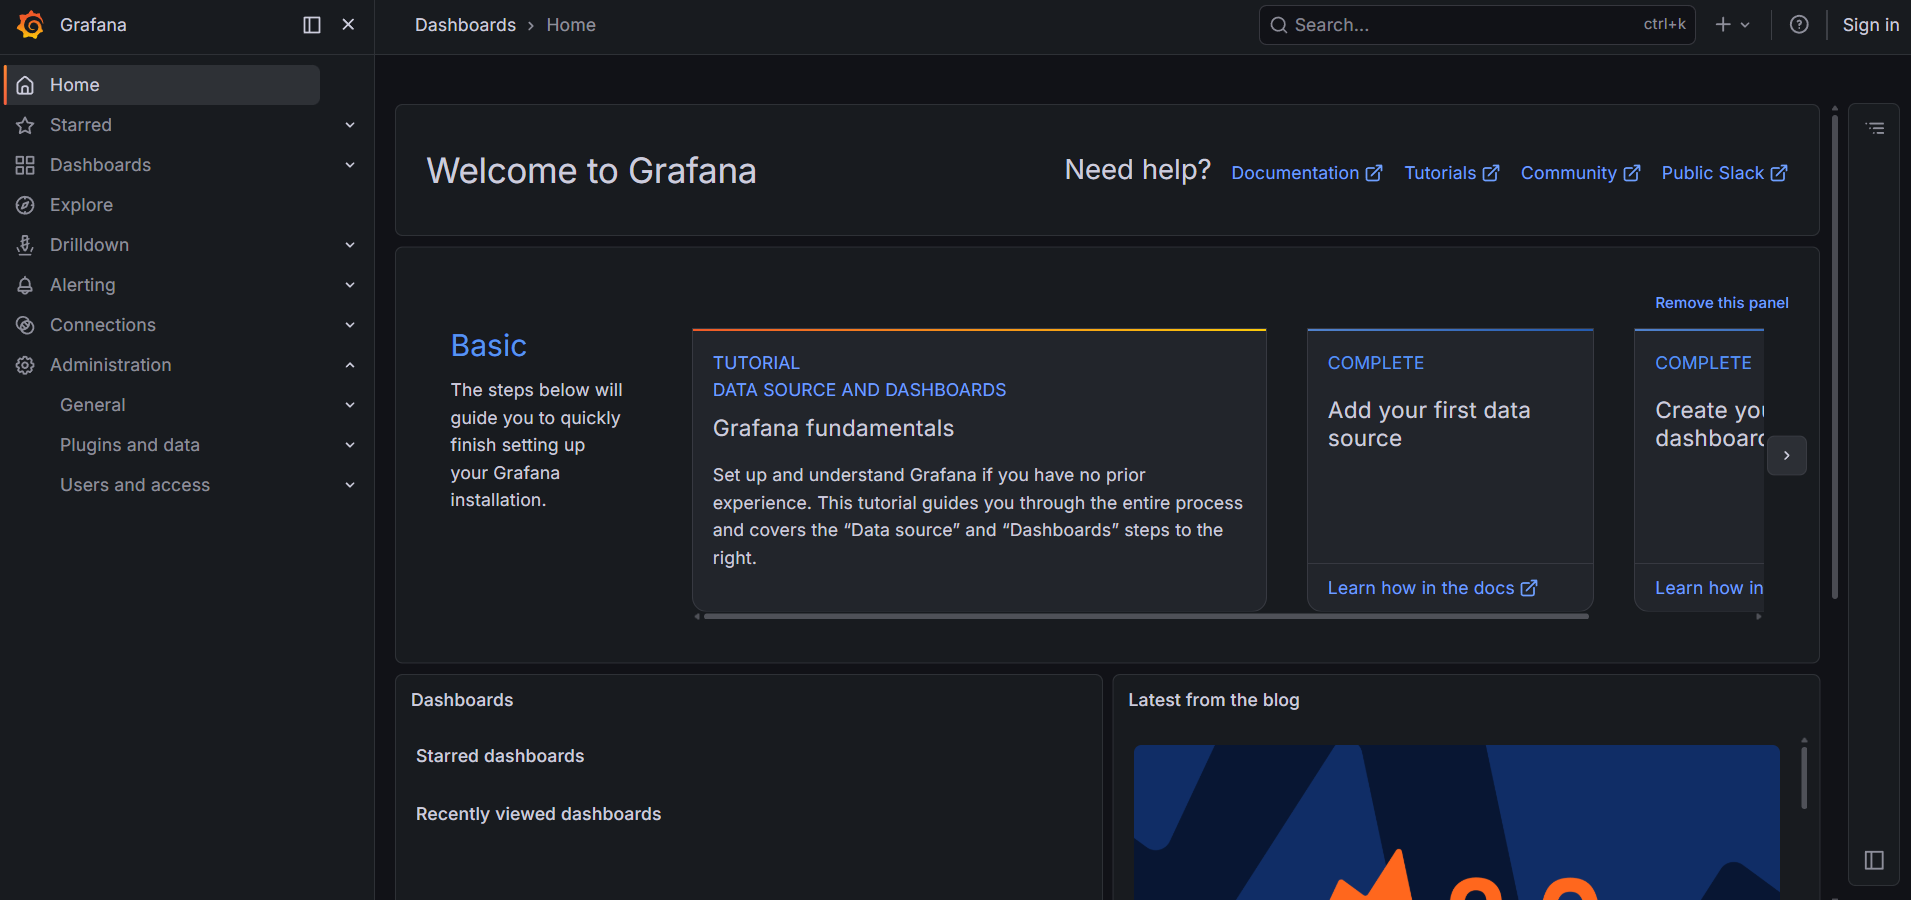
\includegraphics[width=0.9\textwidth]{figures/dashboard-grafana.png}
    \caption{Dashboard de Grafana con los datasources del stack LGTM configurados y recibiendo telemetr\'ia del backend.}
    \label{fig:dashboard-grafana}
\end{figure}

\subsection{Visualizaci\'on de se\~nales}

\begin{figure}[H]
    \centering
    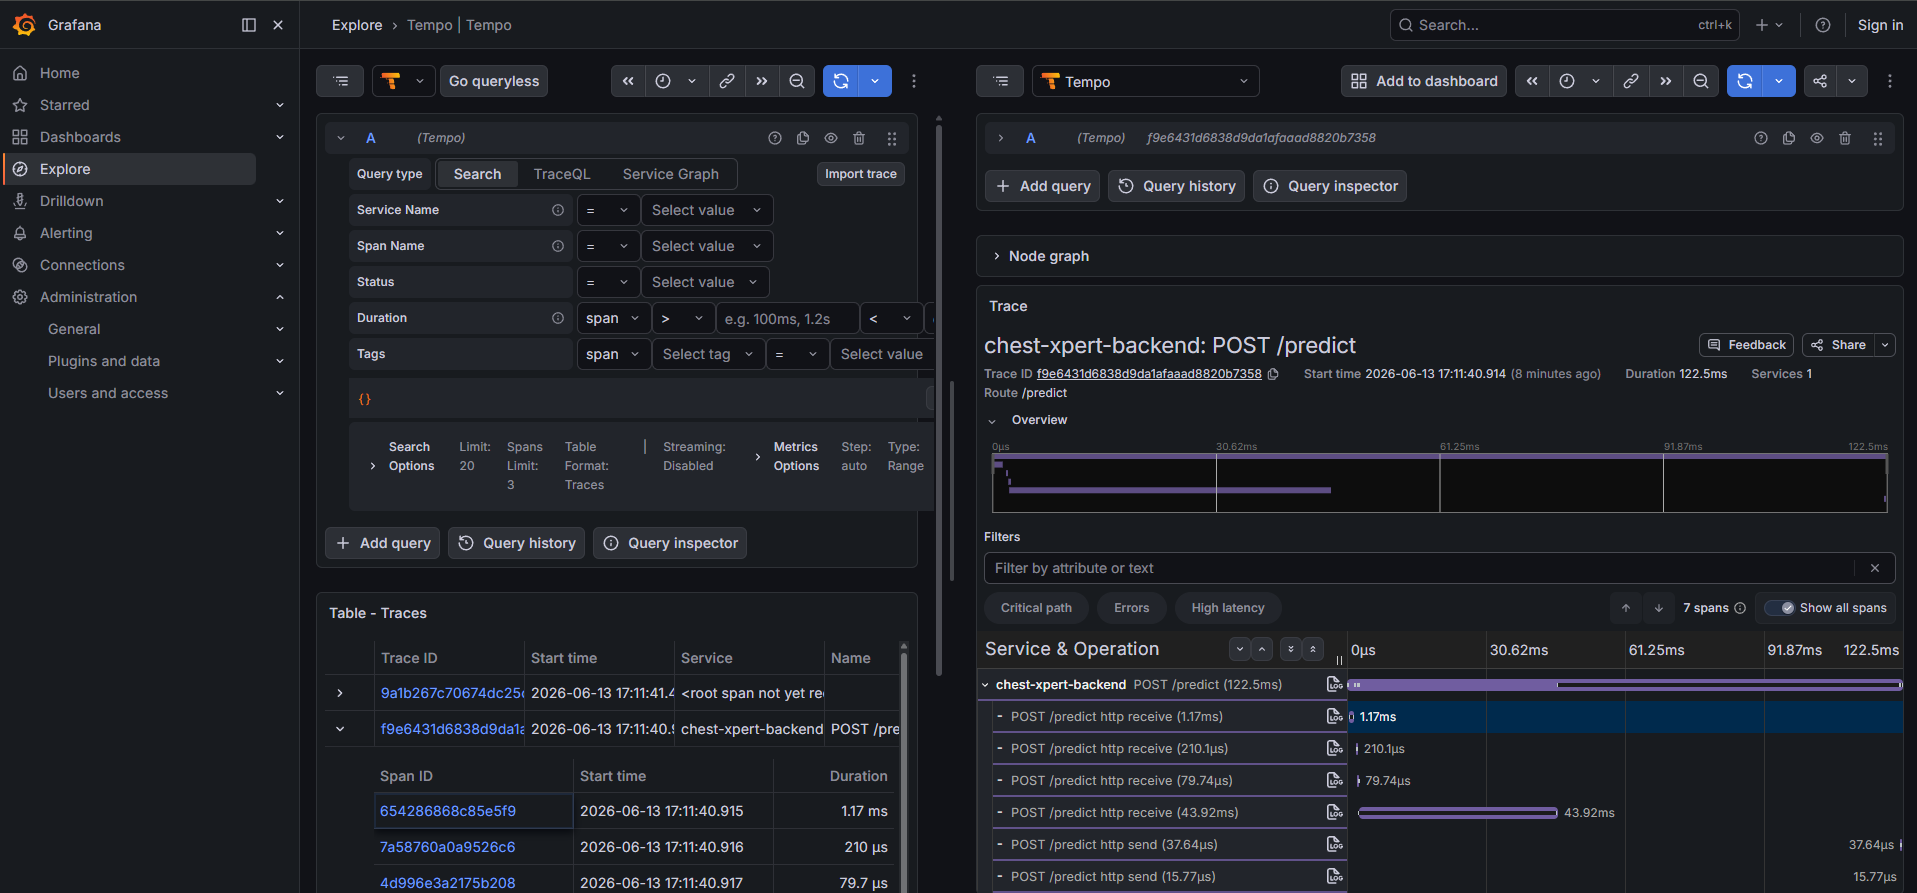
\includegraphics[width=0.9\textwidth]{figures/tempo.png}
    \caption{Tempo: traces distribuidos mostrando latencia por request al endpoint \texttt{/predict}. Cada trace incluye el span completo del ciclo request-response.}
    \label{fig:tempo}
\end{figure}

\begin{figure}[H]
    \centering
    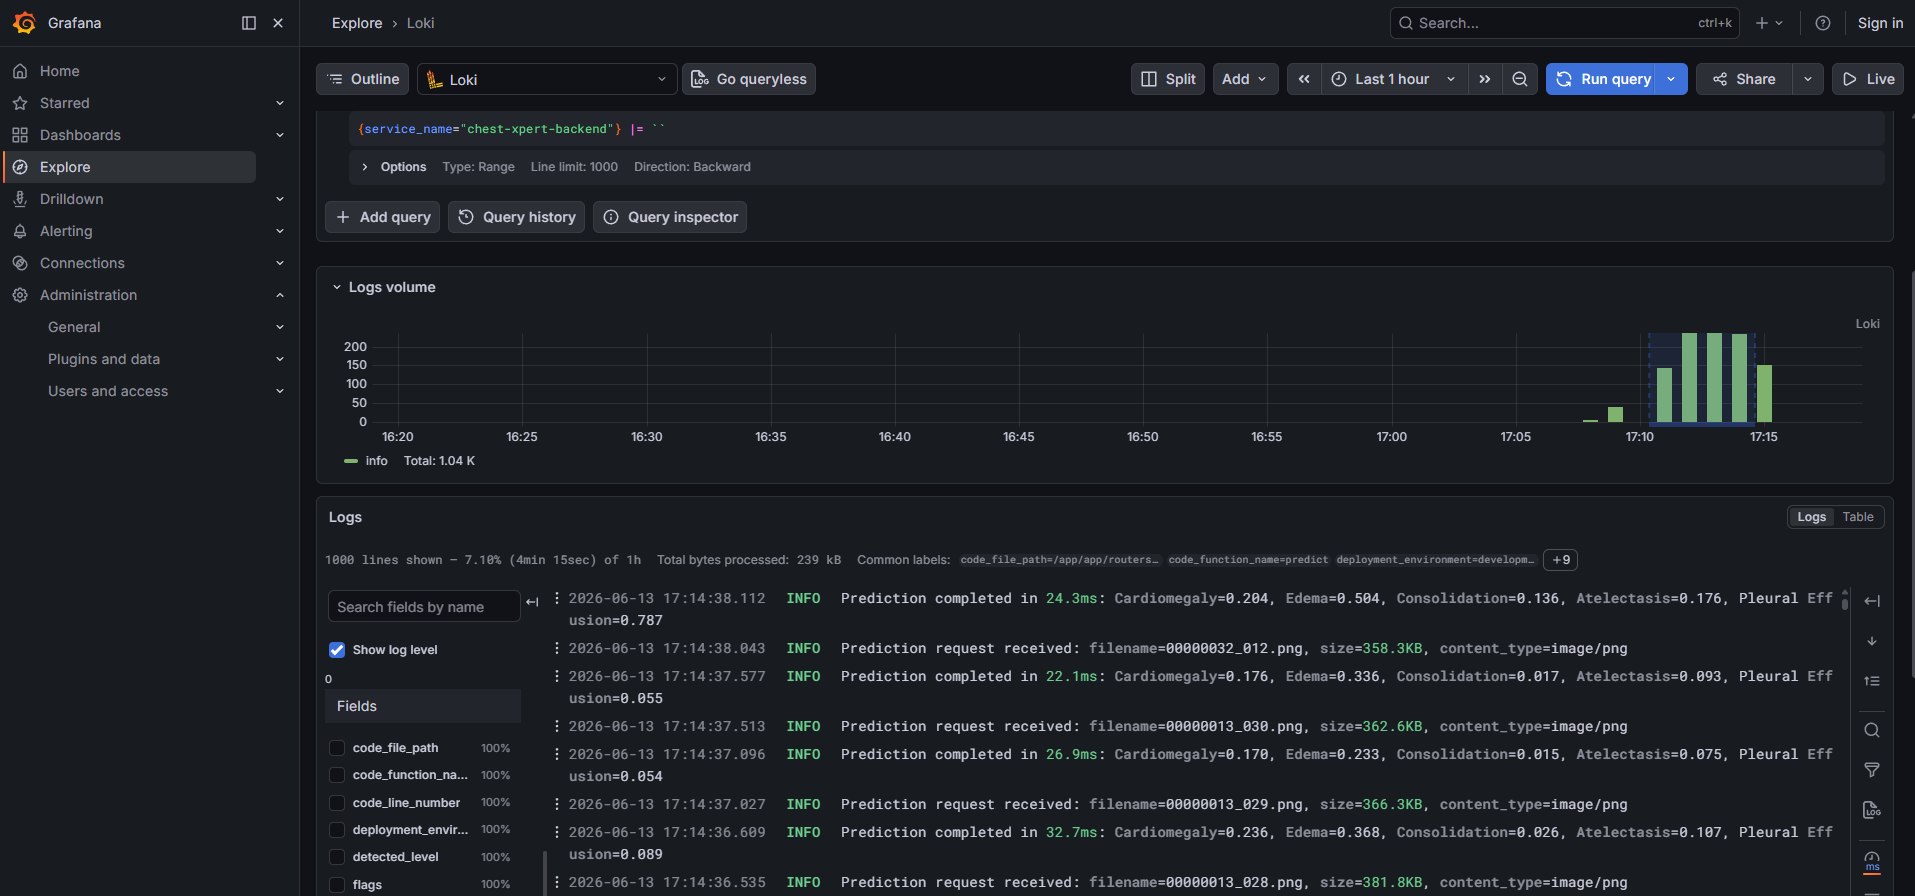
\includegraphics[width=0.9\textwidth]{figures/loki.png}
    \caption{Loki: logs estructurados del backend incluyendo filename, tama\~no, tiempo de inferencia y probabilidades por patolog\'ia.}
    \label{fig:loki}
\end{figure}

\begin{figure}[H]
    \centering
    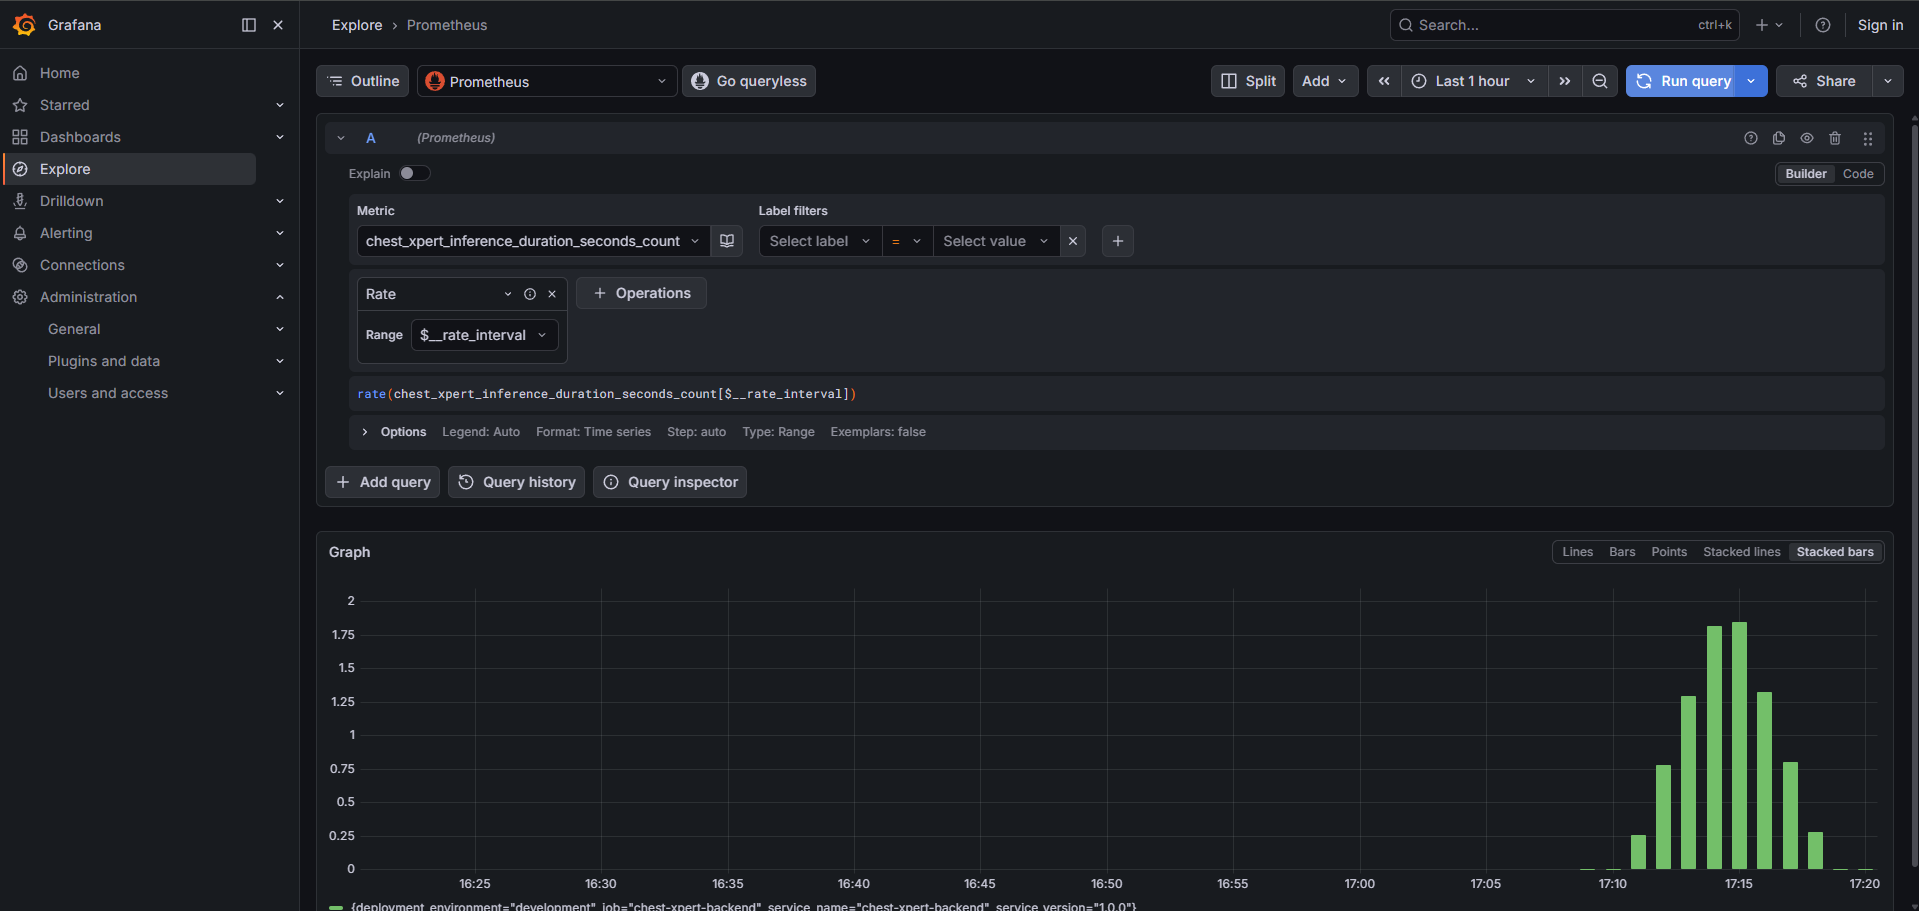
\includegraphics[width=0.9\textwidth]{figures/prometheus.png}
    \caption{Prometheus/Mimir: m\'etricas del servicio incluyendo \texttt{chest\_xpert.predictions\_total} y latencia de inferencia ONNX.}
    \label{fig:prometheus}
\end{figure}

\begin{figure}[H]
    \centering
    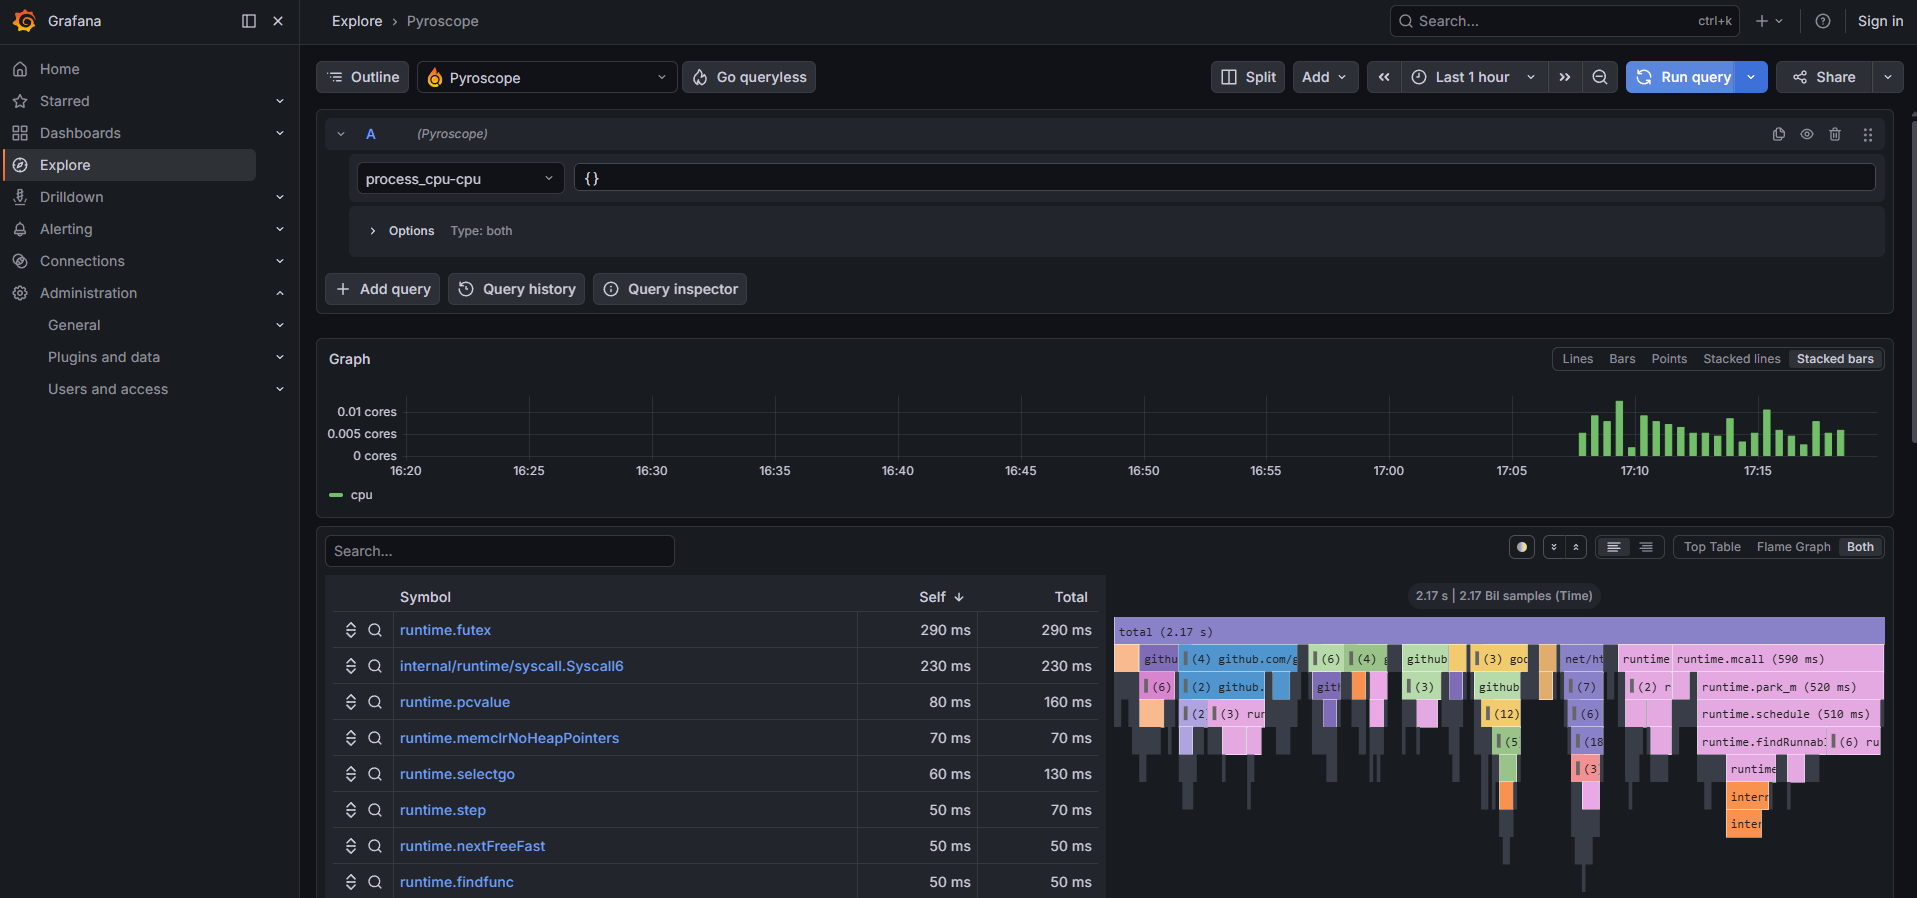
\includegraphics[width=0.9\textwidth]{figures/pyroscope.png}
    \caption{Pyroscope: flame graph de CPU del backend durante carga, permitiendo identificar cuellos de botella en el pipeline de inferencia.}
    \label{fig:pyroscope}
\end{figure}
